\documentclass[conference]{IEEEtran}

\IEEEoverridecommandlockouts

\usepackage{brian}
\usepackage{flushend}

% Bibliography
\usepackage[style=ieee,doi=false,isbn=false,url=false,eprint=false]{biblatex}
\AtEveryBibitem{\clearlist{language}}  % remove language field from bib entries
\addbibresource{references.bib}

\title{\LARGE \bf
    Trajectory Optimization in Maximal Coordinates
}
\vspace{0.25in}
\date{November 2021}

\author{\IEEEauthorblockN{Brian E. Jackson$^*$}
    \IEEEauthorblockA{\textit{Robotics Institute} \\
    \textit{Carnegie Mellon University}\\
    Pittsburgh, USA \\
    brianjackson@cmu.edu}
}

\begin{document}

\maketitle

\begin{abstract}
    Efficiently generating motion plans for systems with inherent sparsity in their 
    dynamics is an outstanding challenge in the robotics community, especially since 
    popular DDP-based approaches do not recognize or exploit this structure. 
    This project explores this topic by solving trajectory optimization problems for 
    rigid body systems represented in maximal coordinates and discrete variational 
    integrators. 
    Trajectory optimization problems for an acrobot and 6 degree-of-freedom robot arm 
    are solved in maximal coordinates. The acrobot trajectories are compared against 
    those generated with a standard direct collocation method using implicit midpoint 
    integration. The results suggest that using Ipopt to solve trajectory optimization 
    problems in maximal coordinates provides no advantage over those expressed minimal 
    coordinates. The solves took many iterations to converge, and frequently failed 
    to converge at all. 
\end{abstract}

\section{Motivation}
In order for autonomous robotic systems to operate sucessfully and robustly in the real 
world, they need to be able to generate and execute motion plans. Ideally, these motion 
plans should be able to balance competing objectives such as time-to-arrival, energy 
efficiency, or safety, handle a broad range of complex scenarios, and be fast to compute
so that new plans may be quickly regenerated as the enviornment around the robot changes.
For robotic systems with few degrees of freedom, such as autonomous cars, quadrotors, planes,
or underwater robots, the task of efficiently generating and following motion plans, at least
for moderately complex scenarios, is relatively straighforward. Approaches to the motion 
planning problem for these systems include sampling-based methods that sample over the 
configuration space of the robot and connect samples based on their feasibility 
\cite{lavalle2001rapidly}, graph-based
methods that discretize the planning space, and optimization-based methods 
\cite{howell_ALTRO_2019,jackson_ALTROC_2021,li_Iterative_2004,hargraves_Direct_1987} that 
discretize and optimize a single planned trajectory. 

While many autonmous systems of interest fall into the previously-mentioned category, many
do not. Multi-body systems such as quadrupeds, humanoids, or robotic manipulators can easily
have between 20-100 degrees of freedom. Moving into distriuted or multi-agent systems such
as power or communication networks, multi-agent teams \cite{jackson_Scalable_2020}, 
satellite constellations, or swarms 
of micro-robots, the dimensionality grows to hundreds of degrees of freedom. And for other
systems, such as soft robotics or fluid control where the fidelity of the system dynamics is
dependent on discretizing a continuous system into a set of finite elements, the number of 
degrees of freedom becomes arbitrarily large. While the dimensionality of the state vectors
describing these systems is often very large, they generally have a unique and sparse coupling
between elements of the state: e.g. links in a robot arm are only connected to 1-3 other 
links via joints, members of a multi-agent team often only communicate locally with the 
robots with a given radius, or finite elements that only couple directly with their 
neighboring elements. When these systems are linearized about some point, this structure 
shows up as sparsity in the underlying matrices, where often 80-99\% of the matrix is zeros,
and only 1-20\% contains meaningful data. Leveraging this inherent sparsity in the system 
dynamics is naturally critical to generating efficient motion plans for these systems.

\begin{figure}[t]
    \centering
    \begin{subfigure}{0.48\columnwidth}
        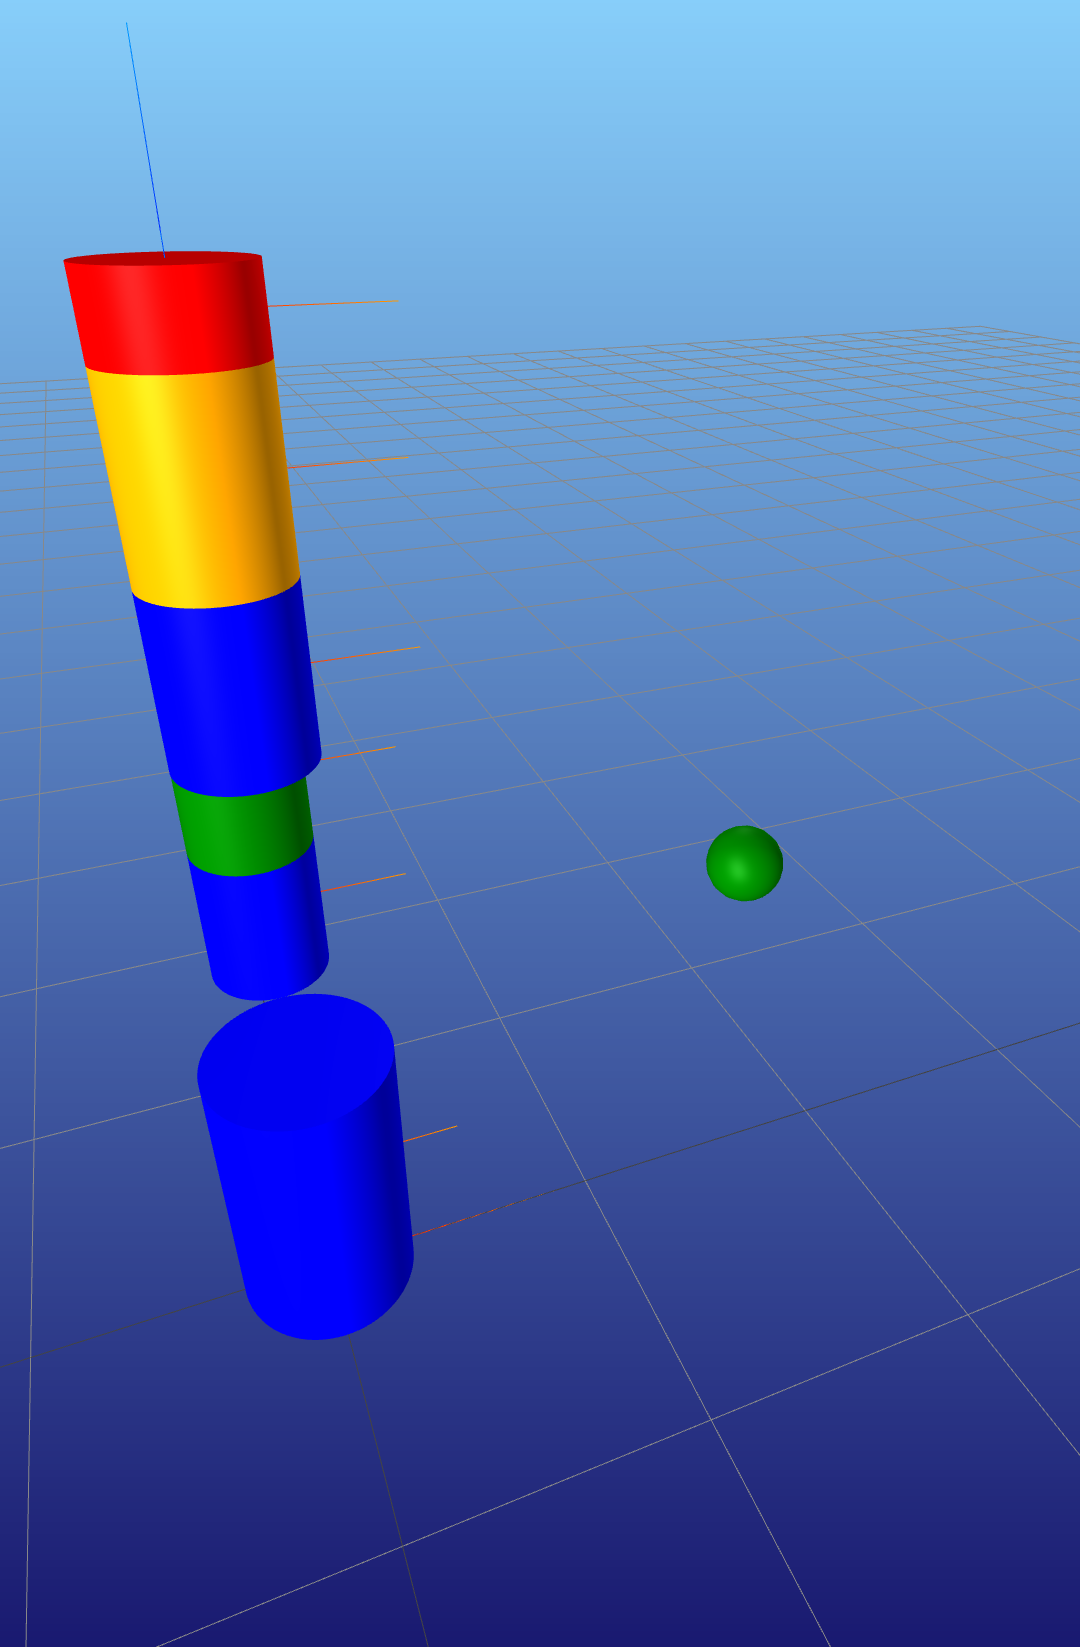
\includegraphics[width=\textwidth]{figs/arm_start.png} 
    \end{subfigure}
    \begin{subfigure}{0.48\columnwidth}
        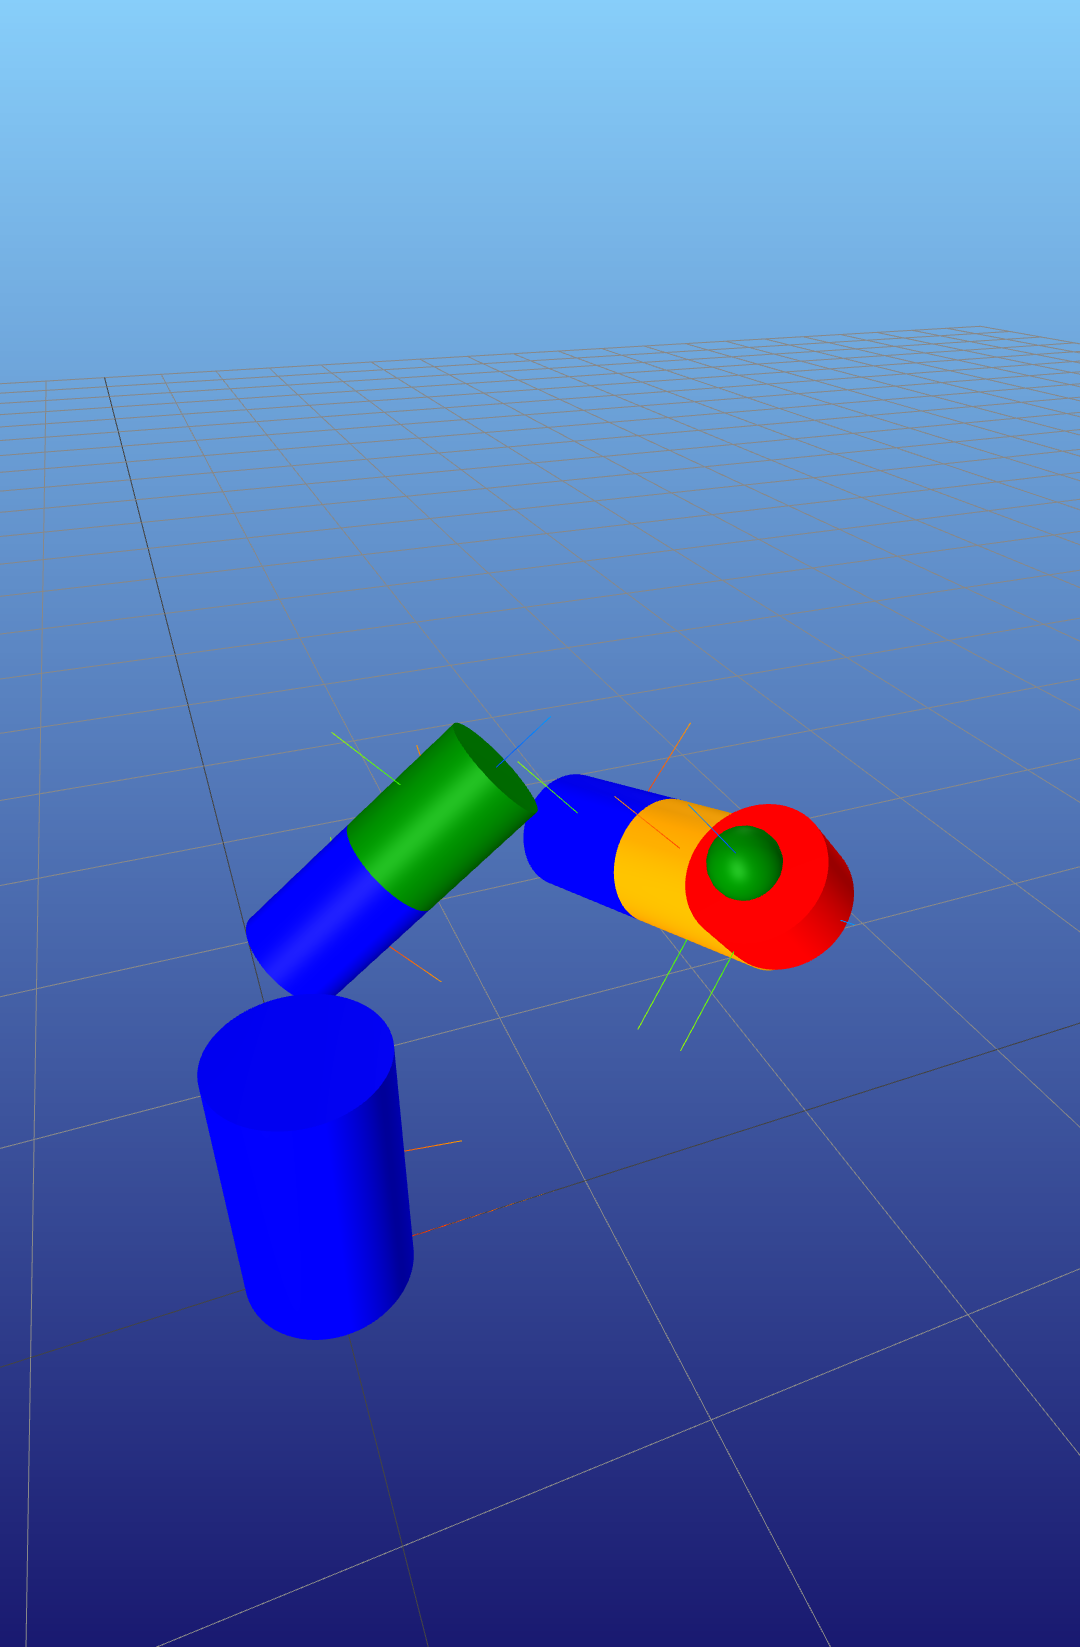
\includegraphics[width=\textwidth]{figs/arm_end.png} 
    \end{subfigure}
    \caption{Arm task of moving from an upright position to a goal location specified in 
        cartesian coordinates. The state and control trajectory was found by solving a 
        trajectory optimization problem in maximal coordinates using Ipopt.
    }
\end{figure}

% While sampling-based and graph-based methods for motion planning work well for systems of 
% few dimensions, they become computationally intractable above a dozen or so dimensions,
% thanks to the infamous ``curse of dimensionality.'' Optimization-based 
% approaches, on the other hand, do not suffer from the same poor scaling properties, and
% large-scale optimization with millions of decision variables is relatively common in the 
% areas of operations research and machine learning. Unlike many of the problems in these 
% areas, which are either formed as well-structured unconstrained nonlinear optimization, 
% problems Linear Programs (LPs), or Quadratic Programs (QPs)---all of which have mature and 
% sophisticated algorithms and software implementations for efficiently solving large 
% optimization problems---optimization-based motion planning problems such as trajectory 
% optimization are nonlinear programs (NLPs) with nonlinear equality constraints that often 
% make the problem extremely difficult to solve. Only a few general-purpose off-the-shelf 
% NLP solvers are commonly used or under active development 
% \cite{wachter_implementation_2006,gill_SNOPT_2005}.

The purpose of this project is to demonstrate the performance of the well-known Ipopt solver
when solving motion planning problems for systems with lots of sparsity in the dynamics. 
In particular, this project focuses on implementing trajetory optimization in maximal 
coordinates using discrete variational integrators. Representing rigid-body systems in 
maximal coordinates has some appealing properties, namely that world or task-based goals 
and constraints, such as the location of an end-effector for manipulation tasks, are 
trivially expressed in maximal coordinates. Additionally, some recent studies have shown
that local control methods such as LQR perform better in maximal coordinate
\cite{brudigam_LinearTime_2020,brudigam2021linear}.  Lastly, by treating a 
mechanism as a finite set of individual rigid bodies linked together by joints, we can 
achieve an extremely high degree of generality and potentially open the door for 
parallelizable algorithms that will hopefully more than offset the cost of solving a larger
optimization problem \cite{baraff_Lineartime_1996}. While some researchers have attempted 
this approach in the past with
dissapointing results \cite{knemeyer2020minor,}, this project leverages state-of-the-art 
variational integrators 
which offer many benefits over the more traditional integration methods used in previous 
studies \cite{manchester_Variational_2017,brudigam_LinearTime_2020,marsden2001discrete}. 
No previous paper has published any sucessful results using this approach, so 
the goal of this paper is to explore the potential of combining maximal coordinates, 
discrete variational integrators, and trajectory optimization.


\section{Background}
\subsection{Rigid Bodies}
A rigid body is a mathematical abstraction that is often extremely useful for describing 
physical systems whose internal dynamics (such as bending modes) are much higher than the 
dynamics of interest. Examples include the structurally stiff links used in classical 
robot manipulators. Many robotic systems are well-approximated by a set of rigid bodies 
held together by joints. For this paper we will deal exclusively with this type of system,
and this section presents the notation and some key equations that arise when dealing with
rigid bodies.

\subsubsection{Rigid Body State}

The state of a rigid body is typically defined by its three-dimensional pose $x \in SE(3)$
and its velocity $v \in TSE(3) \equiv \R^6$. For convenience, we will often split the 
pose and velocity into their translational and rotational components:
\begin{equation}
    x = \begin{bmatrix}
        r \\ q
    \end{bmatrix}, \quad 
    v = \begin{bmatrix}
        \nu \\ \omega     
    \end{bmatrix}
\end{equation}
where $r \in \R^3$ is the position of the body in the world frame, $q \in SE(3)$ is the 
attitude of the body, mapping vectors in the body frame to the world frame, $\nu \in \R^3$ 
is the linear velocity, and $\omega \in \R^3$ is the angular velocity. 

\subsubsection{Attitude Representation}

This project represents the attitude as a quaternion in Hamilton form: 
\begin{equation}
    q = \begin{bmatrix}
        q_s \\ q_v
    \end{bmatrix}
\end{equation}
where $q_s \in \R$ and $q_v \in \R^3$ are the scalar and vector part of the quaternion. 
Although the space of unit quaternions technically represents a double-cover of the space 
of rotations, and our state vector is therefore an element of $\R^3 \times \mathbb{S}^3$,
we will still denote our state vector as element of $SE(3)$ for brevity.
Using the same notation from \cite{jackson_Planning_2021}, we define quaternion 
multiplication as 
\begin{equation}
    q_2 \otimes q_1 = L(q_2) q_1 = R(q_1) q_2
\end{equation}
where $L(q)$ and $R(q)$ are orthonormal matrices defined as:
\begin{equation}
    L(q) = \begin{bmatrix}
        q_s & -q_v^T \\
        q_v & q_s I + \skewmat{q_v}
    \end{bmatrix}
\end{equation}
\begin{equation}
    L(q) = \begin{bmatrix}
        q_s & -q_v^T \\
        q_v & q_s I - \skewmat{q_v}
    \end{bmatrix}
\end{equation}
and $\skewmat{x}$ is the skew-symmetric matrix operator
\begin{equation}
    \skewmat{x} = \begin{bmatrix}
        0   & -x_3 &  x_2 \\
        x_3 & 0    & -x_1 \\
       -x_2 & x_1  &  0
    \end{bmatrix}
\end{equation}

We also define the following matrices for convenience:
\begin{equation}
    T = \begin{bmatrix}
        1 & \\ & -I_3
    \end{bmatrix},
\end{equation}
\begin{equation}
    H = \begin{bmatrix}
        0 \\ I_3
    \end{bmatrix}.
\end{equation}

We denote the rotation matrix defined by a unit quaternion as 
\begin{equation}
    A(q) = H^T L(q) R(q)^T H.
\end{equation}

\subsubsection{Error Pose and Derivatives}
Since our pose is represented with a unit quaternion, we need to account for the unit 
norm constraint when doing common operations like composing states or taking derivatives.
We will frequently need to deal directly with local perturbations about a nominal pose, 
which we denote by the 6-dimensional error pose:
\begin{equation}
    \Delta = \begin{bmatrix}
        \Delta r \\ \Delta \phi
    \end{bmatrix} \in \R^6
\end{equation}
We can convert from an error pose to a normal pose via an exponential map:
\begin{equation}
    \text{exp}(\Delta) = \begin{bmatrix}
        \Delta r \\ \varphi(\Delta \phi)
    \end{bmatrix} \in SE(3)
\end{equation}
where $\varphi(\Delta \phi)$ can be any mapping from a local 3-parameter attitude 
representation to a unit quaternion\footnote{As with the scaled Cayley map used here, 
some care must be taken to ensure the local perturbations are on the scale of radians}. 
For this project, we will use a scaled Cayley map:
\begin{equation}
    q = \varphi(\phi) = \frac{1}{\sqrt{1 + \norm{\half \phi}^2}} \begin{bmatrix}
        1 \\ \half \phi
    \end{bmatrix}
\end{equation}
The scaling is chosen such that the local perturbations have units on the same scale as 
radians. The standard exponential map could also be used, but the Cayley map is more 
computationally efficient. 

Composing two poses is done by adding their translations and multiplying their respective 
quaternions:
\begin{equation}
    r_1 \oplus r_2 = \begin{bmatrix}
        r_1 + r_2 \\ q_1 \otimes q_2
    \end{bmatrix}
\end{equation}

When taking derivatives of functions of poses, we expect the derivatives to be with respect 
to the error pose $\Delta$. Taking the same approach as \cite{jackson_Planning_2021}, we 
get the correct result by differentiating with respect to an error pose composed with the
nominal pose, evaluated with an error pose at the additive identity (i.e. zero):
\begin{align}
    \nabla f(x) &= \pdv{f}{x} \pdv{\Delta}(x \oplus \text{exp}(\Delta)) \Big|_{\Delta = 0} \\
    &= \pdv{f}{x} G(x) = \pdv{f}{x} \begin{bmatrix}
        I_3 & \\ & \half L(q) H
    \end{bmatrix}
\end{align}
where we define $G(x)$ to be the \textit{error pose Jacobian}.

We will also need to differentiate the above equation to obtain second-order derivatives. 
When doing so, we need to evaluate the derivative of $G(x)^T b$ for some vector $b \in \R^4$ 
(usually $\pdv*{f}{x})$. We denote and define this derivative to be:
\begin{equation}
    \nabla G(x,b) = \begin{bmatrix}
        \zeros_3 & \\ & \half H^T R(b) T
    \end{bmatrix}
\end{equation}


\subsection{Trajectory Optimization}
Trajectory optimization is a powerful technique for generating motion plans for complex
autonomous systems. Trajectory optimization generally tries to solve problems of the form:

\begin{mini}[2]
    {x(t), u(t)}{\ell(x(T)) + \int_0^T \ell(x(t), u(t)) dt}{}{}
    \addConstraint{\dot{x}(t) = f(x(t), u(t))}
    \addConstraint{c_E(x(t),u(t)) = 0}
    \addConstraint{c_I(x(t),u(t)) \leq 0}
    \addConstraint{x(0) = x_0}
    \label{opt:trajopt_continuous}
\end{mini}

To compute the solution of these infinite-dimensional optimization problems, we generally 
discretize the trajectories into a set of discrete ``knot points'', and approximate the 
dynamics using some discrete approximation:

\begin{mini}[2]
    {x_{1:N}, u_{1:N}}{\ell(x_N) + \sum_{k=1}^{N-1} \ell(x_k, u_k) }{}{}
    \addConstraint{f_d(x_{k+1}, x_k, u_k), \quad \forall k \in \mathbb{N}_{N-1}}
    \addConstraint{c_E(x_k,u_k) = 0, \quad \forall k \in \mathbb{N}_N}
    \addConstraint{c_I(x_k,u_k) \leq 0, \quad \forall k \in \mathbb{N}_N}
    \addConstraint{x_1 = x_0}
    \label{opt:trajopt}
\end{mini}
where $x \in \R^n, u \in \R^m$ are the state and control vectors, $f_d$ is some 
discrete approximation of the continuous dynamics, and $N$ is the number of knot points. We
define $\mathbb{N}_{i} = 1,\dots,i$ and $\mathbb{N}_{i,j} = i,\dots,j$.

There are many approaches to solving problems of the form \eqref{opt:trajopt}. Differential-
dynamic programming (DDP) \cite{mayne_Secondorder_1966,xie_Differential_2017} and its 
variant iterative LQR (iLQR) \cite{li_Iterative_2004,giftthaler_Family_2017,
farshidian_efficient_2017} are some of the most 
commonly-used methods due to their computational efficiency and relatively straightforward 
implementation. These methods rely on constructing a local quadratic approximation of the 
optimal cost-to-go function, which in general is always dense in the state dimension. This
implies that DDP-based algorithms are poorly-suited to leverage structure (i.e. sparsity)
in the system dynamics.

The other commonly-used method is direct collocation, which traditionally uses 
Hermite-Simpson interpolation to ``transcribe'' the continuous-time problem 
\eqref{opt:trajopt_continuous} into a discrete problem of form \eqref{opt:trajopt}. These 
generally rely on general-purpose NLP solvers like Ipopt \cite{wachter_implementation_2006},
SNOPT \cite{gill_SNOPT_2005}, or Knitro.
Since these solvers all allow the user to provide the sparsity structure of the constraint
Jacobians, they can efficiently leverage sparsity in the dynamics. This project uses 
direct collocation \cite{hargraves_Direct_1987}, but instead of using the traditional 
Hermite-Simpson integration, we use a 2nd-order variational integrator, described in the 
following section. 

\subsection{Variational Integrators}
The dynamics for many robotic systems can be described using the \textit{manipulator equation}:
\begin{equation}
    M(\theta) \ddot{\theta} + C(\theta,\dot{\theta}) + G(\theta) = B(\theta) \tau
\end{equation}
where $\theta \in \R^n$ are generalized coordinates (often joint angles), $M(\theta)$ is 
the mass matrix, 
$C(\theta, \dot{\theta})$ are the Coriolis forces, $G(\theta)$ are the gravitation or 
potential forces, and $B(\theta)$ maps the torques $\tau$ to joint torques. These dynamics
can be discretized by solving for $\ddot{\theta}$ and subsequently using any standard 
quadrature rule, such as a 3rd-order Hermite spline or a 4th-order Runge Kutta method. 

The manipulator equation is the result of applying the famous Euler-Lagrange equation to 
a system of rigid bodies:
\begin{equation}
    \dv{t}(\pdv{L}{\dot{x}}) - \pdv{L}{x} = F(t),
\end{equation}
which itself is just the first-order necessary conditions of the minimum-action principle:
\begin{mini}[2]
    {x(t),v(t)}{\int_0^T L(x(t), v(t)) + F(t)^T x(t)}{}{}
    \addConstraint{\dot{x}(t) = g(v(t))}
    \addConstraint{c(x(t)) = 0}
    \label{opt:minaction}
\end{mini}
where $L(x, v) = T(x,v) - U(x)$ is the Lagrangian, and $K(x,v), U(x)$ are the kinetic
and potential energy of the system. Rather than approximating the discrete dynamics by 
solving \eqref{opt:minaction} to get the Euler-Lagrange equation, which is then approximated
using some integration method, we can instead discretize \eqref{opt:minaction} directly to 
arrive at a discrete version of the Euler-Lagrange equation. This is the central idea behind
discrete mechanics and varitational integrators. In the following section we step through 
the derivation for a 2nd-order variational integrator for systems of rigid bodies.


\section{Discrete Dynamics in Maximal Coordinates}
Assume we have a system of $M$ rigid bodies, each with state $x^{(j)} \in SE(3)$ and velocity 
$v^{(j)} \in \R^6$. The concatenated pose and velocity vectors are denoted in bold face: 
$\mathbf{x} \in M \times SE(3), \mathbf{v} \in \R^{6 \times M}$. Subscript indices are used
to denote time steps.

\subsection{Joint Constraints}
Let the joints of our multi-body system be defined by a directed graph with nodes $1,\dots,M$,
and an edge from $i$ to $j$ denotes a joint between body $i$ and body $j$. The direction 
of the edge provides the convention for applying forces and torques on each body. We assume 
that there is only ever a single edge between a pair of nodes. We denote the graph 
$\mathcal{G}$ with edge set $\mathcal{E}$. The function $\mathcal{N}_1(j)$ returns the
outbound set of vertices from node $j$: $\{i \mid (j,i) \in \mathcal{E}\}$, 
and $\mathcal{N}_2(j)$ likewise returns the inbound set of vertices 
$\{ i \mid (i,j) \in \mathcal{E}\}$. The joint constraint function $c(\mathbf{x})$ is then 
the concatenation of the pairwise joint constraints for each edge in $\mathcal{E}$. For 
this project, we will work only with revolute joints, whose pairwise constraint function is:
\begin{equation}
    c(x^{(1)}, x^{(2)}) = \begin{bmatrix}
        r^{(1)} + A \big( q^{(1)} \big) p_1 - r^{(2)} - A \big( q^{(2)} p_2 \big) \\
        \vec{a}^\perp H^T L(q^{(1)})^T q^{(2)}
    \end{bmatrix}
\end{equation}
where $p_1$ is the location of the joint the link 1 frame, $p_2$ is the location of the 
joint in the link 2 frame, $\vec{a}$ is the axis of rotation as a unit vector in the 
link 1 frame and $\vec{a}^\perp \in \R^{2 \times 3}$ is the orthgonal compliment to the 
joint axis. This is best computed by taking two consecutive cross products with the joint 
axis. 

\subsection{Joint Forces}
Using the same graph as above, we can write functions that provide the forces and torques 
applied to each body by actuating a joint with a torque $u \in \R$ (for revolute joints). 
For each pair of indices in the edge set $\mathcal{E}$ (i.e. each joint) we have two 
functions: 
\begin{subequations}
    \begin{align}
    \xi_1(x^{(1)}, x^{(2)}, u) &= \begin{bmatrix}
        \zeros_{3 \times 1} \\ -\vec{a} \cdot u
    \end{bmatrix} \\
    \xi_2(x^{(1)}, x^{(2)}, u) &= \begin{bmatrix}
        \zeros_{3 \times 1} \\
        A\left(L(q^{(2)})^T q^{(1)}\right) \vec{a} \cdot u
    \end{bmatrix}
    \end{align} 
\end{subequations}
that return the wrenches on link 1 and 2, respectively. The wrench force is defined in the 
world frame and the wrench torque is defined in the body frame of each link.
The total wrench on any link $j$ is then given by the following expression:
\begin{equation} \label{eq:link_wrench}
    \sum_{i \in \mathcal{N}_1(j)} \xi_1\left(x^{(j)}, x^{(i)}, u_j\right) + 
    \sum_{i \in \mathcal{N}_2(j)} \xi_2\left(x^{(i)}, x^{(j)}, u_j\right)
\end{equation}

\subsection{Discrete Dynamics} \label{sec:discrete_dynamics}
If we use midpoint integration on the velocities and position to approximate 
\eqref{opt:minaction} as a sum over discrete terms, we arrive at the \textit{discrete Euler-
Lagrange Equation} (DEL) for a system of rigid bodies:
\begin{equation} \label{eq:DEL_single}
\begin{aligned}
    DEL&(x_1, x_2, x_3, u_1, u_2, \lambda_2) = \\
    &DLT_2(x_1, x_2) + DLT_1(x_2, x_3) \\
    &+ \frac{h}{2} \Bigg( \sum_{\bar{k} = 1}^{2} 
        \sum_{i \in \mathcal{N}_1(j)} \xi_1\left(x_{\bar{k}}^{(j)}, x_{\bar{k}}^{(i)}, u_{\bar{k}}^{(j)}\right) \\
    & + \sum_{i \in \mathcal{N}_2(j)} \xi_2\left(x_{\bar{k}}^{(i)}, x_{\bar{k}}^{(j)}, u_{\bar{k}}^{(j)}\right)
    \Bigg) \\
    & + h \bigg( \sum_{i \in \mathcal{N}_1(j)} \mathbb{D}_1 c\left(x_2^{(j)}, x_2^{(i)}\right)^T \lambda_2^{(ji)} \\
    & +         \sum_{i \in \mathcal{N}_2(j)} \mathbb{D}_2 c\left(x_2^{(i)}, x_2^{(j)}\right)^T \lambda_2^{(ij)} \bigg) = 0
\end{aligned}
\end{equation}
where $DLT_1(x_1, x_2)$ and $DLT_2(x_1, x_2)$ are the left and right 
\textit{discrete Legendre transforms}, respectively. They are derived by taking the 
derivative of \eqref{eq:discrete_lagrangian} with respect to a single pose:
\begin{equation}
    DLT_1(x_1, x_2) = \begin{bmatrix}
        -\frac{m}{h} (r_2 - r_1) - \half h m g e_3 \\
        \frac{4}{h} G(q_1)^T T R(q_2)^T H J H^T L(q_1)^T q_2
    \end{bmatrix}
\end{equation}
\begin{equation}
    DLT_2(x_1, x_2) = \begin{bmatrix}
        \frac{m}{h} (r_2 - r_1) - \half h m g e_3 \\
        \frac{4}{h} G(q_2)^T L(q_1) H J H^T L(q_1)^T q_2
    \end{bmatrix}.
\end{equation}
The derivation of the DEL is provided in more detail in the Appendix. 
We maintain dynamic and kinematic feasibility by enforcing the DEL and the joint constraints 
simultaneously. 

\section{Trajectory Optimization in Maximal Coordinates}
In order to solve trajectory optimization problems in maximal coordinates, we simply 
replace the generic dynamics constraint in \eqref{opt:trajopt} with the discrete 
Euler-Lagrange equation and add the joint constraints. Note that since the DEL is a function
of the joint forces, we need to add those as decision variables to the optimization problem.

Our new trajectory optimization problem is now of the form:
\begin{mini}[3]
    {x_{1:N}^{(1:M)}, u_{1:N-1}, \lambda_{2:N}}{\ell(\mathbf{x}_N) + \sum_{k=1}^{N-1} \ell(\mathbf{x}_k, u_k)}{}{}
    \addConstraint{DEL(x_{k-1}^{(j)}, x_k^{(j)}, x_{k+1}^{(j)}, u_{k-1}, u_k, \lambda) = 0, \quad \forall k \in \mathbb{N}_{2,N-1}}, j \in \mathbb{N}_M
    \addConstraint{c(x_k^{(i)}, x_k^{(j)}) = 0, \quad \forall k \in \mathbb{N}_N, (i,j) \in \mathcal{E}}
    \label{opt:maxcoord_trajopt}
\end{mini}

In order to solve \eqref{opt:maxcoord_trajopt} using Ipopt, we need to supply the constraint
Jacobian with respect to all of the decision variables. Unlike standard forward simulation 
using variational integrators in which only derivatives with respect to $x_3$ are required,
trajectory optimization needs the derivatives with respect to all of the inputs to the DEL
equation. 

\begin{figure}
    \centering
    \begin{subfigure}{0.9\columnwidth}
        \includegraphics[width=\textwidth,height=5cm]{figs/acrobot_eemin.tikz}
        \caption{Minimal Coordinates}
        \label{fig:acrobot_eemin}
    \end{subfigure}
    \begin{subfigure}{0.9\columnwidth}
        \includegraphics[width=\textwidth,height=5cm]{figs/acrobot_eemax.tikz}
        \caption{Maximal Coordinates}
        \label{fig:acrobot_eemax}
    \end{subfigure}
    \label{fig:acrobot_endeffector}
    \caption{End-effector location for acrobot for (a) minimal 
        coordinates, and (b) maximal coordinates. Mark color 
        corresponds to time, with blue being zero seconds and red being the final time.
    }
\end{figure}
\section{Results}
An Ipopt-based solver for trajectory optimization in maximal coordinates was developed from 
scratch in the Julia programming language. For maximal coordinates, automatic differentiation 
was only used for the gradient 
of the cost function: the Jacobian of all constraints were derived and implemented 
analytically. For the minimal coordinate implementation, \texttt{RigidBodyDynamics.jl} was used to 
compute the dynamics and dynamics Jacobians (using automatic differentiation) and the 
dynamics were discretized using implicit 
midpoint integration. All timing results were obtained on an Intel i7-1165G7 processor with
16 GB of memory.

The mass and inertia properties for the double pendulum (acrobot) and robot arm were 
calculated assuming each link was a cylindrical body of aluminum of uniform density of 
2.7 kg/$m^3$.

\subsection{Acrobot}
The acrobot problem is a canonical benchmark problem for generating motion plans for 
underactuated systems. The acrobot is a double pendulum with actuation only at the ``elbow''
joint. This problem was solved using both the maximal coordinate solver and an implementation
of direct collocation in minimal coordinates using implicit midpoint integration.

In addition to the dynamics constraints, both minimal and maximal coordinate solvers 
constrained the end effector to be at the upright position:
\begin{equation}
    r_N^{(M)} + A(q_N^{(M)}) p_\text{ee} - r_\text{goal},
\end{equation}
where $p_\text{ee}$ is the location of the end effector in the last links's frame, and
$r_\text{goal}$ is the location of the goal in the world frame.
For minimal coordinates, $r_N^{(M)}$ and $q_N^{(M)}$ were calculated using forward 
kinematics using \texttt{RigidBodyDynamics.jl}. The objectives for both solvers only 
penalized distance of the end effector to the goal for all time steps, and some 
regularization on the control values, such that they would have identical costs for 
equivalent trajectories. Both solvers were initialized with identical 
initial guesses, which copied the initial state for all states, a control of $5 t$ for 
the time $t$, and the joint forces for the maximal coordinate solver were provided the forces 
obtained by simulating the system forward with the given control inputs. A non-zero control 
input and reasonable estimate of the joint forces were necessary for the solver to converge.

The joint forces from both solvers are shown in Fig. \ref{fig:acrobot_torques}, and the 
objective and constraint violations are shown in Figs. \ref{fig:acrobot_cost} and 
\ref{fig:acrobot_viol}. The end-effector trajectories are shown in Fig. 
\ref{fig:acrobot_endeffector}. In summary, the maximal coordinate solver found a trajectory 
with much lower control torques and therefore got a lower cost. As summarized in Table 
\ref{tab:acrobot}, despite the fact the maximal coordinate trajetory problem is significantly
larger, it's cost per iteration is almost half that of minimal coordinates in this 
preliminary implementation. This is likely due to the fact that evaluating the dynamics Jacobian
in maximal coordinates is extremely simple (not to mention extremely parallelizable) in 
maximal coordinates, whereas minimal coordinates require inverting the mass matrix to solve 
for the accelerations. 

Overall, the maximal coordinate solver was much more brittle than the minimal coordinate 
solver. It took significantly more work to get a good trajectory in maximal coordinates. 
The solver had a tendency to exploit the discretization and ``flip'' the elbow joint in 
one time step, completely violating physical realistic behavior, which could only be 
verified by carefully analyzing the output trajectory. This behavior could be mitigated by 
penalizing the angular velocity of each body, but wasn't used in this example in order to 
keep equivalent cost functions between the two solvers.

\begin{figure}
    \centering
    \includegraphics[width=0.9\columnwidth,height=5cm]{figs/acrobot_torques.tikz}
    \caption{Control torques for the acrobot elbow joint.}
    \label{fig:acrobot_torques}
\end{figure}
\begin{figure}
    \centering
    \includegraphics[width=0.9\columnwidth,height=5cm]{figs/acrobot_cost.tikz}
    \caption{Objective value for acrobot.}
    \label{fig:acrobot_cost}
\end{figure}
\begin{figure}
    \centering
    \includegraphics[width=0.9\columnwidth,height=5cm]{figs/acrobot_viol.tikz}
    \caption{Constraint violations for acrobot.}
    \label{fig:acrobot_viol}
\end{figure}

\begin{table}
    \centering 
    \caption{Min/Max Comparison for Acrobot}
    \begin{tabular}{lcl}
\toprule 
Value & Min Coords & Max Coords \\
\midrule 
Variables & 504 & 2514 \\
Constraints & 403 & 2391 \\
nnz(jac) & 3606 & 45773 \\
Jac density & 1.8\% & 0.8\% \\
Iters & 93.0 & 388.0 \\
Cost & 19683.0 & 429.0 \\
Run time (s) & 6.07 & 11.66 \\
Time/iter (ms) & 65.0 & 125.0 \\
\bottomrule 
\end{tabular}

    \caption*{ \small
        Constraints do not include simple bounds (the initial condition), ``nnz(jac)'' 
        is shorthand for the number of nonzero elements in the constraint Jacobian, and 
        ``Jac density'' is the number of nonzero elements in the constraint Jacobian 
        divided by its total size.
    }
    \label{tab:acrobot}
\end{table}


\subsection{6 DOF Arm}
A simple 6 degree-of-freedom serial-link manipulator was modeled with simlar geometry to the
Kuka iiwa arm. In maximal coordinates, this model has 42 states, 6 controls, and 30 joint 
forces per time step. Similar to the acrobot, the arm was tasked to reach a cartesian point
in the world frame. The objective minimized distance of the end effector to the goal, as 
well as penalizing the linear and angular velocities of each link. The midpoint velocities 
were calculated using the poses at adjacent times steps using the same method described in 
Section \ref{sec:discrete_dynamics}. Gravity was not included in this problem since 
including gravity made it extremely difficult to solve. Future work figuring out a good 
heuristic to do cheap gravity compensation in maximal coordinates should make it easier to
find good trajectories under gravity. 

A summary of the solve is given in Table \ref{tab:arm}. Ipopt produced a high-quality
smooth trajectory (see control torques in Fig. \ref{fig:arm_torques}). While the solver converged
to a high-quality trajectory, it took about 45 seconds to generate, even for this very simple 
point-to-point motion task. 

\begin{table}
    \centering 
    \caption{Summary of Solve for 6DOF Arm}
    \begin{tabular}{lcl}
\toprule 
Value & 6dof Arm \\
\midrule 
Variables & 3942 \\
Constraints & 3567 \\
nnz(jac) & 84269 \\
Jac density & 0.6\% \\
Iters & 235.0 \\
Cost & 140.0 \\
Run time (s) & 39.17 \\
Time/iter (ms) & 167.0 \\
\bottomrule 
\end{tabular}

    \label{tab:arm}
\end{table}

\begin{figure}
    \centering
    \includegraphics[width=0.95\columnwidth,height=5cm]{figs/arm_torques.tikz}
    \caption{Joint torques for the 6 degree-of-freedom arm.}
    \label{fig:arm_torques}
\end{figure}

\section{Conclusion}
This project explored using maximal coordinates to solve trajectory optimization problems.
Although maximal coordinates have some very attractive properties, using them in an 
off-the-shelf solver like Ipopt didn't work very well and doesn't seem to offer any sort of 
advantage over a minimal coordinate representation. It took significant work tuning costs
and providing good initial guesses for the solver to converge. Ipopt frequently got stuck 
in the feasibility restoration phase and claimed infeasibility for some cost values or 
varying initial conditions. While the per-iteration computation time for the acrobot was 
suprisingly fast in maximal coordinates, it usually took many more iterations to converge 
than the minimal coordinate solver. 

Future work could explore writing a custom solver for these types of systems. Since 
satisfying both the discrete Euler-Lagrange and joint constraints is relatively difficult,
some sort of on- or near-manifold optimization method that takes steps that maintain 
dynamic and/or kinematic feasibility between solver iterations could improve convergence. 
A custom NLP solver would also have the advantage of dealing directly the group structure of
quaternions by performing optimization entirely on the error state, rather than adding 
norm constraints to the solver. The code for this project is available at \\
\noindent {\small \url{https://github.com/bjack205/MCTrajOpt}}.


\printbibliography

\appendix
\section{Discrete Euler-Lagrange Equation}
This section provides more details in deriving \eqref{eq:DEL_single}, the 
DEL equation for a system of rigid bodies.

The kinetic and potential energys of our multi-body system are:
\begin{equation}
    T(\mathbf{x},\mathbf{v}) = \sum_{j=1}^M \half (v^{(j)})^T M^{(j)} v^{(j)}
\end{equation}
and the potential energy, under gravity, is:
\begin{equation}
    U(\mathbf{x}) = \sum_{j=1}^M \half m^{(j)} g r_z^{(j)}
\end{equation}


Since the pose of our system lies on a manifold, we must enforce the constraint in 
\eqref{opt:minaction} specifying the state kinematics. We wish to approximate the midpoint 
velocity using two consecutive poses separated by a time step of $h$ seconds. For linear 
velocity, this is just $\frac{1}{2} (r_2 - r_1)$. For angular velocity, we use the quaternion
kinematics:
\begin{equation}
    \dot{q} = \half L(q) H \omega.
\end{equation}
We can approximate the quaternion at the next time step using Euler integration and 
re-arranging to isolate $q_1$, where we use $q_I$ to represent the quaternion identity:
\begin{subequations}
    \begin{align}
        q_{2} &\approx q_1 + h \dot{q}. \\
        q_{2} &\approx q_1 + \frac{h}{2} L(q_1) H \omega. \\
        &\approx L(q_1) q_I + L(q_1) H \left(\frac{h}{2} \omega\right) \\
        &= L(q_1) \left(q_I + H \frac{h}{2} \omega\right)
    \end{align}
\end{subequations}
which we can use to solve for $\omega$ at the midpoint:
\begin{equation}
    \omega = \frac{2}{h} H^T L(q_1)^T q_2
\end{equation}

We can now approximate the continuous-time Lagrangian using two consecutive poses, which we
define as the \textit{discrete Lagrangian}:
\begin{subequations}
    \begin{align}
        L_d(\mathbf{x}_1, \mathbf{x}_2) 
            &= h L(\mathbf{x}_\text{mid}(x_1, x_2), \mathbf{v}_\text{mid}(x_1, x_2)) \\
        = \sum_{j=1}^M &\half W_v(x_1^{(j)}, x_2^{(j)})^T M^{(j)} W_v(x_1^{(j)}, x_2^{(j)}) \nonumber \\
        &- m^{(j)} g e_3^T W_x(x_1^{(j)}, x_2^{(j)}) \label{eq:discrete_lagrangian}
    \end{align}
\end{subequations}
where the pose at the midpoint is approximated as:
\begin{equation} \label{eq:quad_pose}
    W_x(x_1, x_2) = \begin{bmatrix}
        \half (r_1 + r_2) \\ q_1
    \end{bmatrix}
\end{equation}
and the velocity at the midpoint is approximated as:
\begin{equation} \label{eq:quad_vel}
    W_v(x_1, x_2) = \frac{1}{h} \begin{bmatrix}
        (r_2 - r_1) \\ 
        2{h} H^T L(q_1)^T q_2
    \end{bmatrix}
\end{equation}
To achieve higher-order integrators, simply replace these functions with higher-order 
quadrature rules for approximating the pose and velocity along the time step.

Using the similar techniques to those used to convert continuous-time trajectory optimization 
problems \eqref{opt:trajopt_continuous} to a discrete approximation \eqref{opt:trajopt}, we
approximate the continuous-time minimum-action problem \eqref{opt:minaction} that
optimizes over continuous trajectories with a discrete version that optimizes over knot 
points along a trajectory, evenly spaced $h$ seconds apart:
\begin{mini}[2]
    {\mathbf{x}_{1:N}}{\sum_{k=1}^{N-1} L_d(\mathbf{x}_k, \mathbf{x}_{k+1}) + \frac{h}{2}(F_k^T \mathbf{x}_k 
        + F_{k+1}^T \mathbf{x}_{k+1})}{}{}
    % \breakObjective{+ L_d(\mathbf{x}_k, \mathbf{x}_{k+1})}
    \addConstraint{c(\mathbf{x}_k) = 0}
\end{mini}
Here we've decided to enforce the constraints at the knot points instead of the midpoints. 
The pose kinematics constraint has been eliminated since we're handling it implicitly inside
of our quadrature rule \eqref{eq:quad_vel}. 

The first-order necessary conditions for this optimization problem are:
\begin{subequations}
\begin{align}
    &\sum_{k=1}^{N-1} \mathbb{D}_1 L_d(\mathbf{x}_k, \mathbf{x}_{k+1}) \delta \mathbf{x}_k 
     + \mathbb{D}_2 L_d(\mathbf{x}_k, \mathbf{x}_{k+1}) \delta \mathbf{x}_{k+1} \nonumber \\
    &\qquad+\frac{h}{2} F_k^T \delta \mathbf{x}_k
           +\frac{h}{2} F_{k+1}^T \delta \mathbf{x}_{k+1} 
           + h \lambda_k^T \mathbb{D} c(\mathbf{x}_k) = 0 \\
    &c(\mathbf{x}_k) = 0, \forall k \in \mathbb{N}_{N}
\end{align}
\end{subequations}
where $\mathbb{D}_i f(\dots)$ is the partial derivative of $f$ with respect to the $i$th 
argument.

Re-arranging the first condition by removing the $\delta \mathbf{x}_1$ and 
$\delta \mathbf{x}_N$ terms from summation, we get:
\begin{equation}
\begin{aligned}
    &\left(\mathbb{D}_1 L_d(\mathbf{x}_1, \mathbf{x}_2) 
      + F_1^T + h \lambda_1^T \mathbb{D} c(\mathbf{x}_1) 
     \right) \delta \mathbf{x}_1 \\
    & +\sum_{k=2}^{N-1} \Big( \mathbb{D}_2 L_d(\mathbf{x}_{k-1}, \mathbf{x}_k) 
       + \mathbb{D}_1 L_d(\mathbf{x}_{k}, \mathbf{x}_{k+1}) \\
    &   + \frac{h}{2} (F(\mathbf{x}_{k-1}, u_{k-1}) + F(\mathbf{x}_k, u_k))^T 
                     + h \lambda_k^T \mathbb{D} c(\mathbf{x}_k) 
    \Big) \delta \mathbf{x}_k \\
    &+ \left(\mathbb{D}_2 L_d(\mathbf{x}_{N-1}, \mathbf{x}_N) 
     + F_N^T + h \lambda_N^T \mathbb{D}c(\mathbf{x}_N)\right) \delta \mathbf{x}_N = 0. \\
\end{aligned}
\end{equation}
Since $\delta \mathbf{x}_1$ and $\delta \mathbf{x}_N$ are equal to zero 
(no variation at the endpoints), and the summation must be equal to zero for any 
arbitrary $\delta \mathbf{x}_k$, then the terms of the summation must be equal to 0. We now obtain
the \textit{Discrete Euler-Lagrange Equation} (DEL) for a multi-body system:
\begin{multline}
    \mathbb{D}_2^T L_d(\mathbf{x}_{k-1}, \mathbf{x}_k)
       + \mathbb{D}_1^T L_d(\mathbf{x}_{k}, \mathbf{x}_{k+1}) \\
       + \frac{h}{2} (F_{k-1} + F_k) + h \mathbb{D} c(\mathbf{x}_k)^T \lambda_k  = 0.
\end{multline}

Using \eqref{eq:discrete_lagrangian} and \eqref{eq:link_wrench} we can rewrite the DEL for
each individual link, which results in Equation \eqref{eq:DEL_single}.

\end{document}